\documentclass{article}
\usepackage{tikz}
\usetikzlibrary{matrix, positioning}
\usepackage{xcolor}
\usepackage{amsmath}
\usetikzlibrary{positioning, arrows.meta}
\usetikzlibrary{calc}
\usepackage{pgfplots}

% Define background and text colors
\definecolor{bgcolor}{RGB}{27, 27, 27}
\definecolor{textcolor}{RGB}{255, 255, 255}

\pagecolor{bgcolor}
\color{textcolor}
\usepackage{textpos}

\usepackage[paperwidth=16in, paperheight=9in, margin=0cm]{geometry}




\begin{document}
\pagenumbering{gobble} % No page numbers

\begin{textblock*}{\textwidth}(0cm,2cm) % Adjust position (x, y) here
    \centering


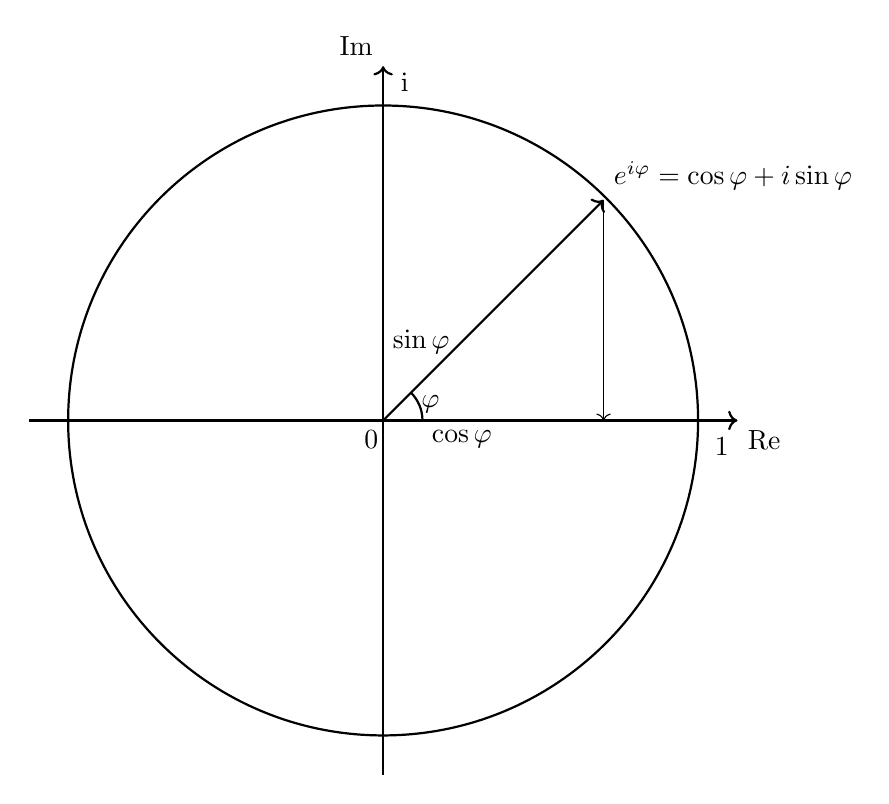
\begin{tikzpicture}
    % Draw the unit circle
    \draw[thick] (0,0) circle (4cm);
    
    % Draw the axes
    \draw[->, thick] (-4.5,0) -- (4.5,0) node[anchor=north west] {Re};
    \draw[->, thick] (0,-4.5) -- (0,4.5) node[anchor=south east] {Im};
    
    % Draw the angle and the complex exponential
    \draw[->, thick] (0,0) -- (2.8,2.8) node[above right] {$e^{i\varphi} = \cos \varphi + i \sin \varphi$};
    \draw[->, thin] (2.8,2.8) -- (2.8,0);
    
    % Draw the cosine and sine projections
    \node[anchor=north] at (1,0) {$\cos \varphi$};
    \node[anchor=west] at (0,1) {$\sin \varphi$};
    
    % Draw labels for 0, 1, and i
    \node[anchor=north] at (4.3,-0.1) {1};
    \node[anchor=north] at (-0.15,-0.0) {0};
    \node[anchor=west] at (0.1,4.3) {i};
    
    % Draw the angle arc
    \draw[thick] (0.5,0) arc (0:45:0.5);
    \node at (0.6,0.2) {$\varphi$};
\end{tikzpicture}

\end{textblock*}

\begin{textblock*}{\textwidth}(0cm,12cm)
\centering

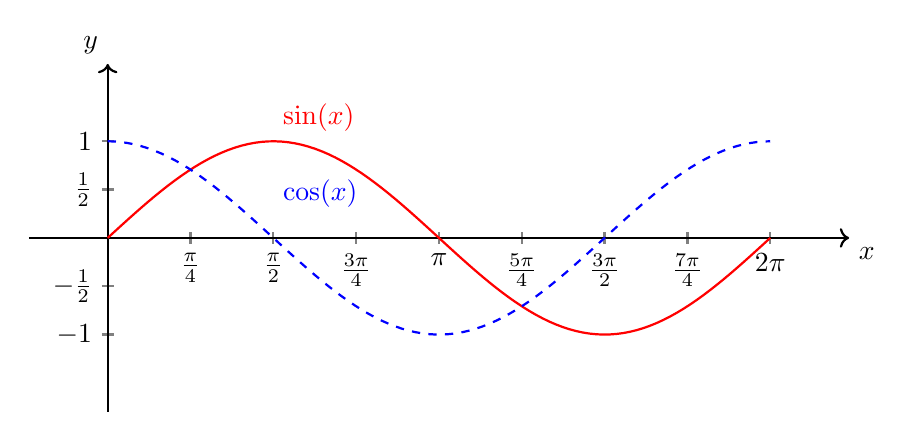
\begin{tikzpicture}
    \begin{axis}[
        axis lines=middle,
        enlargelimits,
        xtick={0, pi/4, pi/2, 3*pi/4, pi, 5*pi/4, 3*pi/2, 7*pi/4, 2*pi},
        xticklabels={$0$, $\frac{\pi}{4}$, $\frac{\pi}{2}$, $\frac{3\pi}{4}$, $\pi$, $\frac{5\pi}{4}$, $\frac{3\pi}{2}$, $\frac{7\pi}{4}$, $2\pi$},
        ytick={-1, -1/2, 0, 1/2, 1},
        yticklabels={$-1$, $-\frac{1}{2}$, $0$, $\frac{1}{2}$, $1$},
        xlabel={$x$},
        ylabel={$y$},
        ymin=-1.5, ymax=1.5,
        xmin=-0.1, xmax=2*pi + 0.1,
        axis line style={->, thick},
        tick style={thick},
        x label style={below right},
        y label style={above left},
        width=12cm,
        height=6cm
    ]
    % Plot sine curve
    \addplot[domain=0:2*pi, samples=100, red, thick] {sin(deg(x))};
    \node[above right, red] at (axis cs: pi/2, 1) {$\sin(x)$};
    
    % Plot cosine curve
    \addplot[domain=0:2*pi, samples=100, blue, thick, dashed] {cos(deg(x))};
    \node[below right, blue] at (axis cs: pi/2, 0.7) {$\cos(x)$};
    \end{axis}
\end{tikzpicture}
\end{textblock*}

% \begin{textblock*}{\textwidth}(0cm,17.5cm) % Center textblock
% \centering % Center the equations within the block
% \Large 
% $\Delta v = v_e \text{ln} \frac{m_0}{m_f}=I_{\text{sp}} g_0 \text{ln}\frac{m_0}{m_f}$

% \vspace{10pt} % Add spacing between equations if needed

% $v = \sqrt{\frac{2GM}{r}}$
% \end{textblock*}

\end{document}
